\documentclass[10pt]{beamer}

\mode<presentation> 
{ \usetheme[nat,dogma]{Frederiksberg} }

% \usepackage[danish]{babel}
\usepackage[latin1]{inputenc}
\usepackage{times}
\usepackage[T1]{fontenc}
\usepackage[english]{babel}
\usepackage{hyperref}
\usepackage{animate}
%\usepackage{multimedia}
\usepackage{francois-preamble}
\usepackage{multirow}

\usepackage{multirow}
%\usepackage{movie15}

\newcommand{\cc}{{c\!\!,}}
\newcommand{\degr}[1]{{{#1}^\circ}}

\title{Vision and Image Processing:\\ Camera Models}

\author[F.~Lauze] % (optional, use only with lots of authors)
{Fran{\c c}ois Lauze}

\institute[DIKU] % (optional, but mostly needed)
{
  Department of Computer Science\\
  University of Copenhagen
}

\date[2013-14 B2] % (optional, should be abbreviation of conference name)
% {Research Presentation, Diku 2006}

\definecolor{gold}{rgb}{0.95,0.83,0.0}
\definecolor{orange}{rgb}{0.95,0.7,0.0}
% \definecolor{backblue}{rgb}{0.93,0.94,0.99}
\definecolor{backblue}{rgb}{0.95,0.94,0.99}
\setbeamercolor*{background canvas}{bg=backblue} 



\newcommand{\myemph}[1]{{\color{blue}{#1}}}
\newcommand{\intrg}[1]{\int_{{#1}=-\infty}^\infty}
\newcommand{\intRR}{\int_{-\infty}^\infty}

\AtBeginSection[]
{
  \begin{frame}<beamer>{Outline}
    \tableofcontents[currentsection,currentsubsection]
  \end{frame}
}

\begin{document}
\maketitle

% would be cool with more images showing applications


%-------------------------------------------------------------------
%   Start slides
%-------------------------------------------------------------------




%----------------------------------------------



\begin{frame}
  \frametitle{Plan for today}
  \begin{itemize}
  \item Before we start: vectors and matrices.
  \item Motivation and a bit of history.
  \item A general Introduction to Camera Models, specifically the pinhole model.
  \item Notions of projection and projective geometry
  \item 2 Views and Epipolar Geometry.
  \end{itemize}
\end{frame}


\section{Vectors and Matrices}

\begin{frame}
  \frametitle{Vectors}
  \begin{itemize}
  \item A $n$-vector is a $n$-uple of real values:
    $$
    v =
    \begin{pmatrix}
      x_1\\\dots\\x_n
    \end{pmatrix}
    $$
  \item Addition
    $$
    \begin{pmatrix}
      x_1\\\vdots\\x_n
    \end{pmatrix}
    +
    \begin{pmatrix}
      y_1\\\vdots\\y_n
    \end{pmatrix}
    =
    \begin{pmatrix}
      x_1+y_1\\\vdots\\x_n+y_n
    \end{pmatrix}
    $$
  \item Multiplication by a scalar
    $$
    \lambda\begin{pmatrix}
      x_1\\\vdots\\x_n
    \end{pmatrix}
    = 
    \begin{pmatrix}
      \lambda x_1\\\vdots\\\lambda x_n
    \end{pmatrix}
    $$
  \end{itemize}
\end{frame}


\begin{frame}
  \frametitle{Linear Mapping}
  \begin{itemize}
  \item Mapping between vectors with only addition of coordinates, multiplications by scalar and no constant terms.
  \item Example
    $$
    f
    \begin{pmatrix}
      x\\y\\z
    \end{pmatrix}
    =
    \begin{pmatrix}
      x+3y\\z-2x
    \end{pmatrix}
    $$
  \item Non linear example
    $$g
    \begin{pmatrix}
      x\\y\\z
    \end{pmatrix}
    =
    \begin{pmatrix}
      x^2+3yz\\z-2x^2 + 1
    \end{pmatrix}
    $$
    There are powers and constant terms.
  \end{itemize}
\end{frame}

\begin{frame}
  \frametitle{Linearity}
  \begin{itemize}
  \item This means $f(v+ \lambda v') = f(v) + \lambda f(v')$
    \begin{align*}
     f\left(
    \begin{pmatrix}
      x\\y\\z
    \end{pmatrix}+\lambda
    \begin{pmatrix}
      x'\\y'\\z'
    \end{pmatrix}
    \right)
    &= f
    \begin{pmatrix}
      x+\lambda x'\\y+\lambda y'\\z+\lambda z'
    \end{pmatrix}\\
    &=
    \begin{pmatrix}
      x+\lambda x'+3(y+\lambda y')\\
      z+\lambda z'-2(x+\lambda x')
    \end{pmatrix}\\
    &=
    \begin{pmatrix}
      x+3y\\
      z-2x\\
    \end{pmatrix}
    +\lambda 
    \begin{pmatrix}
      x'+3y'\\
      z'-2x'
    \end{pmatrix}\\
    &= f
    \begin{pmatrix}
      x\\y\\z
    \end{pmatrix}
    + \lambda f
    \begin{pmatrix}
      x'\\y'\\z'
    \end{pmatrix}
  \end{align*}
\item $f$ is linear.
\end{itemize}
\end{frame}

\begin{frame}
  \frametitle{Matrices}
  \begin{itemize}
  \item A $n\times m$ matrix is an array of numbers with $n$ rows and $m$ columns
  \item A 2$\times 3$ matrix $F$
    $$
    F =
    \begin{pmatrix}
      1 & 3 & 0\\
      -2 & 0 & 1
    \end{pmatrix}
    $$
  \item 2 matrices \myemph{of the same size} can be added together: just add the entries:
    $$    
    \begin{pmatrix}
      1 & 3 & 0\\
      -2 & 0 & 1
    \end{pmatrix}+
    \begin{pmatrix}
      4 & -2 & 1\\
      7 & -3 & 0
    \end{pmatrix}
    =
    \text{ ? }
    $$
  \end{itemize}
\end{frame}


\begin{frame}
  \frametitle{Product of a Matrix and a Vector}
  \begin{itemize}
  \item A matrix of size $m\times n$ and a vector of length $m$ can be multiplied to form a vector of length $n$.
  \item Formal rule:
    $$
    A =
    \begin{pmatrix}
      a_{11}&\dots& a_{1m}\\
      \vdots & \vdots & \vdots\\
      a_{n1}&\dots& a_{nm}\\
    \end{pmatrix},
    v =
    \begin{pmatrix}
      v_1\\\vdots\\ v_n
    \end{pmatrix}
    $$
    $$
    A v =
    \begin{pmatrix}
      a_{11} v_1 + a_{12}v_2 + \dots a_{1m} v_n\\
      a_{21} v_1 + a_{22}v_2 + \dots a_{2m} v_n\\
      \vdots\\
      a_{n1} v_1 + a_{n2}v_2 + \dots a_{mn} v_n\\
    \end{pmatrix}
    $$
    \item Each line of $A$ is multiplied in ``inner product way'' with $v$.
  \end{itemize}
\end{frame}


\begin{frame}
  \begin{itemize}
  \item Example: Compute the product of 
    $$
    A =
    \begin{pmatrix}
        1 & 3 & 0\\
      -2 & 0 & 1
    \end{pmatrix}\text{ and }
    v =
    \begin{pmatrix}
      x\\y\\z
    \end{pmatrix}
    $$
    \pause
  \item We find precisely the value of 
    $$   
    f
    \begin{pmatrix}
      x\\y\\z
    \end{pmatrix}
    =
    \begin{pmatrix}
      x+3y\\-2x+z
    \end{pmatrix}=
    \begin{pmatrix}
      x+3y\\z-2x
    \end{pmatrix}
    $$
  \item Each linear mapping can be written that way. Often use the same notation for the matrix and the linear mapping.
  \end{itemize}
\end{frame}



\begin{frame}
  \frametitle{Matrices /linear mappings as geometric transformations}. 
  \begin{columns}
    \column{0.5\textwidth}
    \begin{center}
    Projection  on $x-y$ plane
    \end{center}
    \column{0.5\textwidth}
    
\includegraphics[width=\textwidth]{FIGURES/3dto2dproj}
  \end{columns}
  \begin{center}
    \includegraphics[width=0.9\textwidth]{FIGURES/simpletransforms}\\
    Rotation of angle $\theta$ \hfill anisotropic scaling \hfill ~~~~~~shear~~~~~~~~~~~
  \end{center}
\end{frame}

\begin{frame}
  \begin{itemize}
  \item projection $\RR^3\to\RR^2$
    $$
    F
    \begin{pmatrix}
      x \\y \\z
    \end{pmatrix}
    =
    \begin{pmatrix}
      x \\y
    \end{pmatrix},\quad F =
    \begin{pmatrix}
      1 & 0 & 0\\
      0 & 1 & 0\\
      0 & 0 & 0
    \end{pmatrix}
    $$
  \item Rotation of angle $\theta$ from $\RR^2\to\RR^2$:
    $$
    R_\theta
    \begin{pmatrix}
      x \\y
    \end{pmatrix}
    =
    \begin{pmatrix}
      x\cos\theta - y\sin\theta\\
      x\sin\theta + y\cos\theta
    \end{pmatrix},\quad
    R_\theta =
    \begin{pmatrix}
      \cos\theta & -\sin\theta\\
      \sin\theta & \cos\theta
    \end{pmatrix}
    $$
  \item Scaling by a factor $\alpha$ in $x$ and $\beta$ in $y$:
    $$
    S
    \begin{pmatrix}
     x\\y 
    \end{pmatrix}
    = 
    \begin{pmatrix}
      \alpha x\\
      \beta y
    \end{pmatrix},\quad
    S =
    \begin{pmatrix}
      \alpha & 0\\0 & \beta
    \end{pmatrix}
    $$
  \item Shear of the $y$-axis with  angle $\theta$:
    $$
    \Ss
    \begin{pmatrix}
      x\\y
    \end{pmatrix}
    =
    \begin{pmatrix}
      x + \sin\theta y\\
      y
    \end{pmatrix},\quad
    \Ss =
    \begin{pmatrix}
      1 &\sin\theta\\
      0 & 1
    \end{pmatrix}
    $$
  \end{itemize}
\end{frame}



\begin{frame}
  \frametitle{Product of Matrices}
  \begin{itemize}
  \item A matrix of size $m\times n$ and a matrix of size $n\times p$
    can be multiplied to produce a matrix of size $m\times p$.
  \item Algebraic rule: $a_{ij}$ entry $(i,j)$ of $A$, $b_{jk}$ entry $(j,k)$ of $B$
    $$
    A = (a_{ij})_{\substack{i=1\dots m\\j=1\dots n}},\quad 
    B = (b_{jk})_{\substack{j=1\dots n\\k=1\dots p}}
    $$
    Denote entry $(i,k)$ of product $C = AB$ by $c_{ik}$:
    $$
    c_{ik} = \sum_{j = 1}^n a_{ij}b_{jk}
    $$
  \item Matrix vector multiplication is in fact a special case of it!
  \item Example
    $$
    \begin{pmatrix}
      2 & 2\\
      1 & 3\\
      1 & -1\\
    \end{pmatrix}
    \begin{pmatrix}
      1 & 3 & 0\\
      -2 & 0 & 1
    \end{pmatrix}
    = \onslide<2->
    \begin{pmatrix}
      -2 & 6 & 2\\
      -5 & 3 & 3\\
      3 & 3 & -1
    \end{pmatrix}
    $$
  \item What does matrix multiplication means?
  \end{itemize}
\end{frame}

\begin{frame}
  \frametitle{Meaning of the Product}
  \begin{itemize}
  \item $M$ and $N$ the linear mappings $
    \begin{pmatrix}
      2 & 2\\
      1 & 3\\
      1 & -1\\
    \end{pmatrix}
    $ and 
    $
    \begin{pmatrix}
      1 & 3 & 0\\
      -2 & 0 & 1
    \end{pmatrix}
    $
  \item
    Apply $N$ to $
    \bv = \begin{pmatrix}
      x \\ y \\ z
    \end{pmatrix}
    $
    and $M$ to the result:
    $$
    N \bv = \begin{pmatrix}
      1 & 3 & 0\\
      -2 & 0 & 1
    \end{pmatrix}\begin{pmatrix}
      x \\ y \\ z
    \end{pmatrix}
    = 
    \begin{pmatrix}
      x + 3y\\
      -2x + z
    \end{pmatrix}
    $$
    \item and{\small
      $$
      \begin{pmatrix}
      2 & 2\\
      1 & 3\\
      1 & -1\\
    \end{pmatrix}
     \begin{pmatrix}
      x + 3y\\
      -2x + z
    \end{pmatrix}
    =\onslide<2->
    \begin{pmatrix}
      -2x+6y+2z\\
      -5x + 3y+3z\\
      3x + 3y-z
    \end{pmatrix}
    =\onslide<3->
    \begin{pmatrix}
      -2 & 6 & 2\\
      -5 & 3 & 3\\
      3 & 3 & -1
    \end{pmatrix}
    \begin{pmatrix}
      x\\y\\z
    \end{pmatrix}
    $$}
    % \item VIP (Very Important Property) \myemph{Matrix multiplication correspomds to chaining linear transforms}!
  \end{itemize}
\end{frame}


\begin{frame}
  \frametitle{Matrix Product as Chain Application of Linear Mappings}
  \begin{itemize}
  \item We found that 
    $$
    M\left (N\bv\right) = \udesc{\text{Matrix product}}{M N}\bv
    $$
  \item Very Important Property: Matrix product corresponds to chain application (composition) of linear mappings!
  \end{itemize}\vfill
  \begin{center}
    \large
    Read the Linear Algebra Tutorial and Reference on Absalon!   
  \end{center}
  This will also be useful for other courses!
\end{frame}


\section{Introduction}

\begin{frame}
  \frametitle{Motivation}
  \begin{center}
    \includegraphics[width=\textwidth]{IMAGES/trocadero_annotations}
  \end{center}
\end{frame}


\begin{frame}
  \frametitle{Questions}
  Previous picture raises some questions about:\vfill
  \begin{itemize}
  \item Lines?
  \item Parallelism?
  \item Angles / orthogonality?
  \item Sizes?
  \item Camera position / Horizon?\vfill
  \end{itemize}
  What happens when you take a picture (or Daphn{\'e} Haour-Hidalgo in the previous case :-))
\end{frame}


\section{The Pinhole Camera}

\begin{frame}
  \frametitle{Getting an Image -- I}
  \begin{center}
    \includegraphics[width=0.55\textwidth]{FIGURES/oliphantnopinhole}
  \end{center}
  Many rays emanating from the same position touch the image sensitive
  array at many location: big blur!
\end{frame}


\begin{frame}
  \frametitle{Getting an Image -- II}
  \begin{center}
    
\includegraphics[width=0.65\textwidth]{FIGURES/oliphantpinhole}
  \end{center}
  Filtering the rays via a pinhole: get an (inverted) image. Principle
  of the \myemph{Camera Obscura} (dark room).
\end{frame}

\section{A bit of History}


\begin{frame}
  \frametitle{Camera Obscura}
  \begin{center}
    \begin{tabular}[h]{cc}
      \includegraphics[width=0.4\textwidth]{IMAGES/WMCamera_obscura_box} &
      \includegraphics[width=0.4\textwidth]{IMAGES/WMCameraObscura18thCentury}\\
      Principle of Camera Obscura & 18th Century Camera Obscura
    \end{tabular}
  \end{center}
  \begin{itemize}
  \item Known from old chines writings
  \item Mentioned by Aristotle
  \item Plaque with photosensitive material: Photographic camera!
  \end{itemize}
\end{frame}

\begin{frame}
  \frametitle{The Very First Photography, 1826}
  \begin{center}
    \includegraphics[width=0.8\textwidth]{IMAGES/WindowLegrasNiepce}
  \end{center}
  J.N. Ni�pce, View from the window at Le Gras,
  Saint Loup de Varennes, France -- Now at University of Texas at
  Austin.
\end{frame}


\begin{frame}
  
  \begin{center}
    \frametitle{The Pioneers}
    \begin{tabular}[h]{ccc}
      \includegraphics[width=0.3\textwidth]{IMAGES/JNNiepce} &
      \includegraphics[width=0.3\textwidth]{IMAGES/LDaguerre} &
      \includegraphics[width=0.3\textwidth]{IMAGES/HFTalbot} \\
      J. Nic�phore Ni�pce & Louis Daguerre & Henri F. Talbot
    \end{tabular}
  \end{center}
\end{frame}


\begin{frame}
  \frametitle{Now...}
  \begin{center}
    \includegraphics[width=0.8\textwidth]{IMAGES/smartphonecamera}
  \end{center}
\end{frame}



\section{Projection}


\begin{frame}
  \frametitle{The Pinhole Camera Model}
  \begin{center}
    \includegraphics[width=0.9\textwidth]{FIGURES/coproj}
  \end{center}
  \begin{itemize}
  \item $f$ is the focal length,
  \item $O$ is the camera center.
  \end{itemize}
\end{frame}


\begin{frame}
  \frametitle{Projection is Tricky!}
  \begin{center}
    \includegraphics[width=0.8\textwidth]{IMAGES/shigeoFukuda}
  \end{center}
  Some illusions from Shigeo Fukuda. 
\end{frame}




\begin{frame}
  \frametitle{Perspective Effects}
  Remember from Kim's first lecture
  \begin{center}
    \includegraphics[width=0.9\textwidth]{FIGURES/fp131}
  \end{center}
  Far objects appear smaller that close ones.
\end{frame}


\begin{frame}
  \frametitle{Perspective Effects}
  Remember from Kim's first lecture again
  \begin{center}
    \includegraphics[width=0.9\textwidth]{FIGURES/fp132}
  \end{center}
  Images of parallel lines intersect at the horizon (virtual image plane).
\end{frame}





\begin{frame}
  \frametitle{Projection Equations}
  \begin{center}
    \includegraphics[width=0.9\textwidth]{FIGURES/fp14}
  \end{center}
  \begin{itemize}
  \item  $P (x,y,z)$, $P' (x',y',z')$. $P'$ in the image plane $\implies z' = f$
  \item Remember optical flow lecture: similar triangles:
    $$
    x' = f\frac{x}{z},\quad y' = f\frac{y}{z}
    $$
  \end{itemize}
\end{frame}




\begin{frame}
  \frametitle{Lost in projection}
    \begin{center}
    \includegraphics[width=0.8\textwidth]{IMAGES/trocadero_annotations}
  \end{center}
  Angles, size, parallelism.
\end{frame}


\begin{frame}
  \frametitle{Preserved by projection}
    \begin{center}
    \includegraphics[width=0.8\textwidth]{IMAGES/trocadero_annotations}
  \end{center}
  Straight lines.
\end{frame}

\begin{frame}
  \frametitle{Vanishing Points}
    \begin{center}
    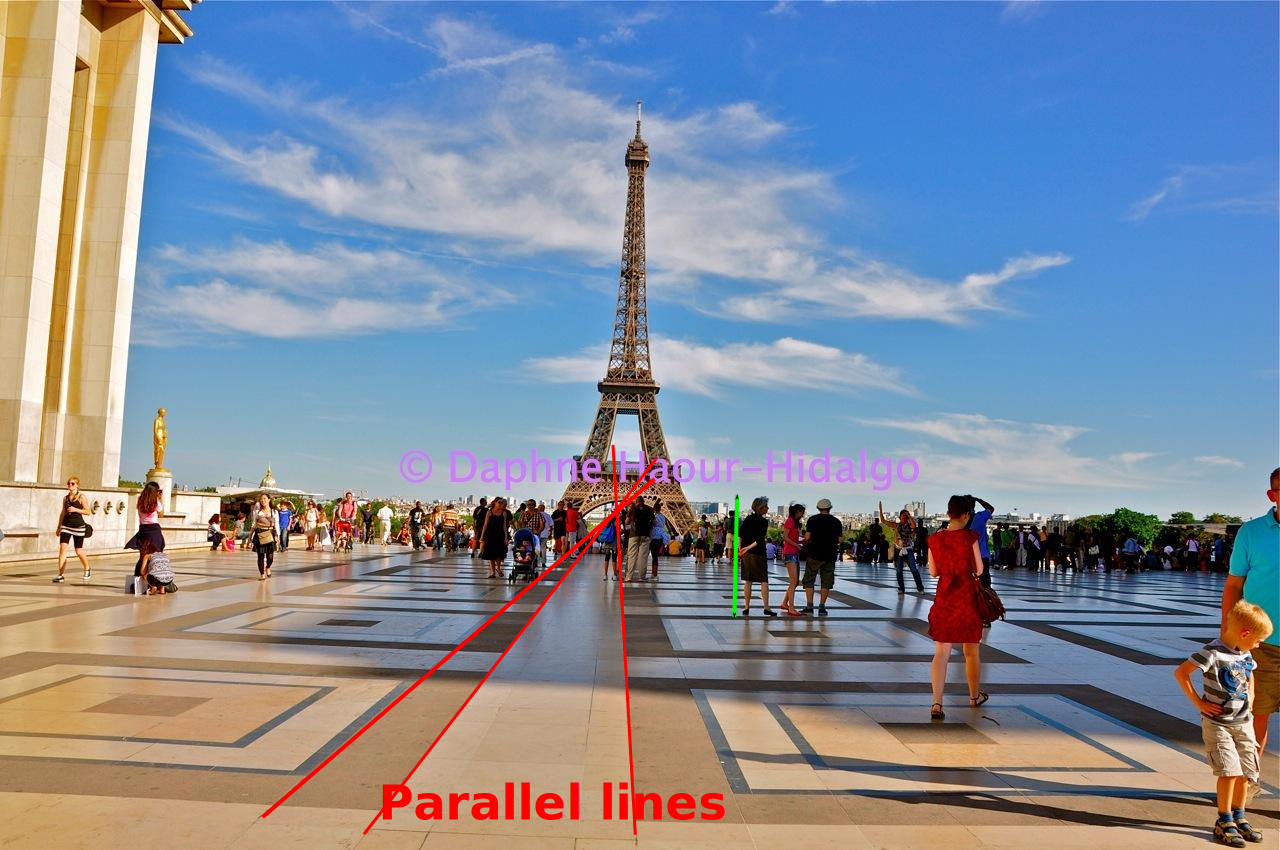
\includegraphics[width=0.8\textwidth]{IMAGES/trocaderolines}
  \end{center}
  Projections of parallel lines intersect at common points.
\end{frame}

\begin{frame}
  \frametitle{Vanishing line}
  \begin{center}
    \includegraphics[width=0.8\textwidth]{FIGURES/vanishingline}
  \end{center}
  Vanishing points intersect at a common line. Intersection can be at infinity.
\end{frame}

\begin{frame}
  \frametitle{Homogeneous coordinates 1D}
  {\small
  \begin{itemize}
  \item In 1D coordinate is just 1 number. 
    \begin{center}
      
\includegraphics[width=0.75\textwidth]{FIGURES/1dcoords}
    \end{center}
  \item 1D coordinate to 1D Homogeneous coordinates: 
    $$x\sim
    \begin{bmatrix}
      x\\1
    \end{bmatrix}
    $$
  \item 1D homogeneous coordinate to 1 D coordinate
    $$
     \begin{bmatrix}
      x\\w
    \end{bmatrix}\sim x/w 
    $$
  \item What can we do with that? we can ``tame'' infinity!
  \item A point with homogeneous coordinate $[x,0]^T$ has ``normal'' coordinate $x/0 = \infty$
    as if we took homogeneous coordinate $[\infty,1]^T$
    \begin{center}
      
\includegraphics[width=0.75\textwidth]{FIGURES/1dcoordshomog}
    \end{center}
  \end{itemize}
  }
\end{frame}





\begin{frame}
  \frametitle{Homogeneous coordinates, 2D}
  ``Natural Coordinates'' for projective geometry
  \begin{itemize}
  \item From 2D point coordinate to 2D Homogeneous coordinate
    $$
    (x,y)\Implies
    \begin{bmatrix}
      x\\y\\1
    \end{bmatrix}
    $$
  \item From 2D homogeneous coordinates to 2D coordinates
    $$   
    \begin{bmatrix}
      x\\y\\w
    \end{bmatrix}
    \Implies 
    (x/w, y/w)
    $$
  \item Exercise: $P$ with coordinates $(x,y,1)$. $Q(x',y',w)$ point
    on the line through $O (0,0,0)$ and $P$.  Compute $x'$ and $y'$.
    Considering $[x',y',w]$ as homogeneous 2D coordinates, what are
    the corresponding 2D coordinates?
  \end{itemize}
\end{frame}


\begin{frame}
  \frametitle{Homogeneous coordinates, 3D}
  \begin{itemize}
  \item From 3D point coordinate to 3D Homogeneous coordinate
    $$
    (x,y,z)\Implies
    \begin{bmatrix}
      x\\y\\z\\1
    \end{bmatrix}
    $$
  \item From 3D homogeneous coordinates to 3D coordinates
    $$   
    \begin{bmatrix}
      x\\y\\z\\w
    \end{bmatrix}
    \Implies 
    (x/w, y/w, z/w)
    $$
  \end{itemize}
\end{frame}

\begin{frame}
  \frametitle{Homogeneous coordinates}
  \begin{center}
    
\includegraphics[width=0.7\textwidth]{FIGURES/projcoords1}
  \end{center}
  Homogeneous coordinates in 2D correspond to points in plane $z=1$
  but also to lines through the origin and this point.
\end{frame}

\begin{frame}
  \frametitle{Why Are They Useful}
  \begin{itemize}
  \item Projection to image plane in standard coordinates:
    $$
    P: (x,y,z)\mapsto P': (f\frac{x}{z}, f\frac{y}{z})
    $$
  \item In homogeneous coordinates:\pause
    $$
    P:
    \begin{bmatrix}
      x\\y\\z\\1
    \end{bmatrix}
    \mapsto P': 
    \begin{bmatrix}
      fx\\fy\\z
    \end{bmatrix}
    $$
  \item Matrix notation
    $$
     \begin{bmatrix}
      fx\\fy\\z
    \end{bmatrix}
    = \udesc{M}{
    \begin{pmatrix}
      f & 0 & 0 & 0\\
      0 & f & 0 & 0\\
      0 & 0 & 1 & 0
    \end{pmatrix}}
    \begin{bmatrix}
      x\\y\\z\\1
    \end{bmatrix}
    $$
    \item $M$ is the \myemph{Camera Matrix}
  \end{itemize}
\end{frame}


\begin{frame}
  \frametitle{World,Camera and Image Coordinates}
  In the previous slides, Many coordinate systems are implicitly known:
  \begin{itemize}
  \item 3D World Coordinates: Coordinate system of the 3D world.
  \item Camera Coordinates: 3D coordinate system attached to the camera.
  \item Image Coordinates: 2D Coordinate system attached to the image plane.
  \end{itemize}
  Not that simple in practice!
\end{frame}

\begin{frame}
  \frametitle{Assumptions Behind the Simple Model}
  \begin{center}
    \includegraphics[width=0.9\textwidth]{FIGURES/fp14}
  \end{center}
  \begin{itemize}
    \item The camera center $0$ is the same as the world coordinates origin,
    \item The axes $\bi$, $\bj$ and $\bk$ are common for the camera and the world
    \item Pixels are squared and perfectly aligned with the camera coordinates.
    \item Image coordinates have their origin at $C'$, projection of the camera center $O$.
  \end{itemize}
\end{frame}


\begin{frame}
  \frametitle{Intrinsic vs Extrinsic Camera Parameters}
  Intrinsic parameters refer to internal parameters:
  \begin{itemize}
  \item Position of the image center wrt projection of the camera center: 2 parameters
  \item Scale factors for the pixels sizes in both x and y directions: 2 parameters,
  \item Skewness of pixels: 1 parameter.
  \end{itemize}
  Extrinsic Camera parameters refer
  \begin{itemize}
  \item position of the camera coordinate system vs the world coordinates system:
    translation,
  \item orientation of the camera coordinate system vs the world coordinates system:
    rotation.
  \end{itemize}
\end{frame}


\begin{frame}
  \frametitle{Oriented and Translated Camera}
  \begin{center}
    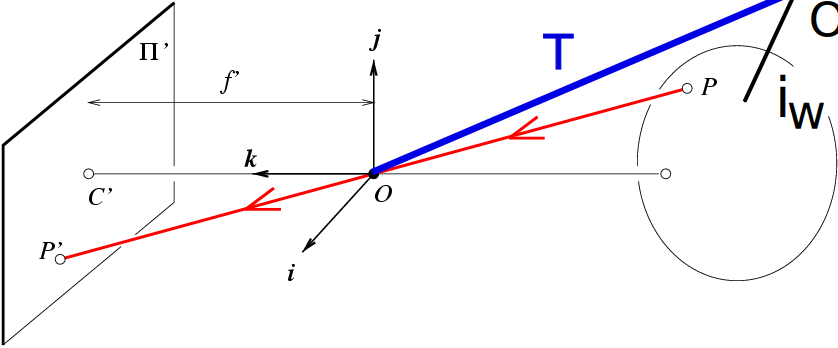
\includegraphics[width=0.9\textwidth]{FIGURES/orientedtranslatedcam1}
  \end{center}
\end{frame}

\begin{frame}
  \frametitle{Translating Coordinate System}
  \begin{center}
   
\includegraphics[width=0.9\textwidth]{FIGURES/translation3D} 
  \end{center}
  Assume $O'$ at coordinates $(x_{O'},y_{O'},z_{O'})$ in coordinate system
  $(O,\bi,\bj,\bk)$ and $P$ has coordinates $(x,y,z)$ also in $(O,\bi,\bj,\bk)$.
  What are its coordinates in $(O',\bi,\bj,\bk)$?
 \end{frame}


 \begin{frame}
   \begin{itemize}
   \item Let $(x',y',z')$ its coordinates in $(O,\bi,\bj,\bk)$.
   \item Write $\overrightarrow{O'P}$ = $\overrightarrow{OP} - \overrightarrow{OO'}$
   \item Develop:
     $$
     \begin{pmatrix}
       x'\\y'\\z'
     \end{pmatrix}
     = 
     \begin{pmatrix}
       x\\y\\z
     \end{pmatrix}
     -
     \begin{pmatrix}
       x_{O'}\\y_{O'}\\z_{O'}
     \end{pmatrix}
     =
     \begin{pmatrix}
       x-x_{O'}\\y-y_{O'}\\z-z_{O'}
     \end{pmatrix}
     $$
   \item Transformation in homogeneous coordinates:
     $$
     \begin{bmatrix}
       x'\\y'\\z'\\1
     \end{bmatrix}
     =
     \begin{pmatrix}
       1 & 0 & 0 & -x_{O'}\\
       0 & 1 & 0 & -y_{O'}\\
       0 & 0 & 1 & -z_{O'}\\
       0 & 0 & 0 & 1
     \end{pmatrix}
     \begin{bmatrix}
       x\\y\\z\\1
     \end{bmatrix}
     $$
   \end{itemize}
 \end{frame}


 \begin{frame}
   \frametitle{Rotating Coordinate System}
   \begin{columns}
     \column{0.5\textwidth}
     \begin{center}
       \includegraphics[width=\textwidth]{FIGURES/rotation3d}
     \end{center}
     \column{0.5\textwidth}
     Rotations along coordinate axes
     $$
     R_{x\alpha} = 
     \begin{pmatrix}
       1 & 0 & 0\\
       0 & \cos\alpha & -\sin\alpha\\
       0 & \sin\alpha & \cos\alpha
     \end{pmatrix}
     $$
     $$
     R_{y\beta} = 
     \begin{pmatrix}
       \cos\beta & 0 & -\sin\beta\\
       0 & 1 & 0\\
       \sin\beta & 0 & \cos\beta
     \end{pmatrix}
     $$
     $$ 
     R_{y\gamma} = 
     \begin{pmatrix}
       \cos\gamma & -\sin\gamma & 0\\
       \sin\gamma & \cos\gamma & 0\\
       0 & 0 & 1
     \end{pmatrix}
     $$
   \end{columns}~\\
   ~\\
   Can also be written in homogeneous coordinates
 \end{frame}
 
 \begin{frame}
   \frametitle{Camera Matrix}
   \begin{itemize}
   \item Combine world vs camera coordinates with
   \item Simple Camera matrix and 
   \item Image plane transformation (axis scalings, shear, translation)
     $$
     {\bf C} = {\bf K} \left[{\bf  R}\,\, {\bf t}\right]
     $$
   \item ${\bf K}$ $3\times 3$ matrix encoding the homogeneous transformations
     inside the camera: \myemph{calibration matrix}.
   \item $\left[{\bf R}\,\, {\bf t}\right]$ Concatenation of world
     coordinates rotation and origin translation to align camera and
     world coordinates.
   \end{itemize}
   $$
   w
   \begin{bmatrix}
     u\\b\\1
   \end{bmatrix}
   = \udesc{{\bf K}}{
     \begin{pmatrix}
       \alpha & s & u_0\\
       0 & \beta & v_0\\
       0 & 0 & 1
     \end{pmatrix}}
   \udesc{\left[{\bf R}\,\, {\bf t}\right]}{
     \begin{pmatrix}
       r_{11} & r_{12} & r_{13} & t_x\\
       r_{21} & r_{22} & r_{23} & t_y\\
       r_{31} & r_{32} & r_{33} & t_z\\
     \end{pmatrix}}
   \begin{pmatrix}
     x\\y\\z\\1
   \end{pmatrix}
   $$
 \end{frame}
 

 \begin{frame}
   \frametitle{Geometric Calibration}
   \begin{itemize}
     \item Computing the camera matrix is called geometric calibration.
     \item Extrinsic parameters: usually easy.
     \item Calibration focuses more on intrinsic parameters (calibration matrix ${\bf K}$).
     \item Often difficult.
   \end{itemize}
   \begin{columns}
     \column{0.5\textwidth}
     \begin{center}
       \includegraphics[width=0.8\textwidth]{IMAGES/calibrationobject}
     \end{center}
     \column{0.5\textwidth}
     \begin{itemize}
     \item Use an object with known geometry
     \item Use vanishing points / lines
     \item Use other cues...
     \end{itemize}
   \end{columns}
 \end{frame}


 \begin{frame}
   \begin{center}
     \includegraphics[width=0.8\textwidth]{IMAGES/amesroom}
   \end{center}
   Without knowledge of object geometry, calibration can be very problematic (Ames Room illusion).
 \end{frame}


\section{More on Camera Models}


\begin{frame}
  \frametitle{Shrinking the aperture}
  \begin{center}
    \includegraphics[width=0.7\textwidth]{IMAGES/shrinkingaperture}
  \end{center}
  Less light in, diffraction. 
\end{frame}


\begin{frame}
  \frametitle{Adding Lens}
   \begin{center}
    \includegraphics[width=0.7\textwidth]{FIGURES/addinglens}
  \end{center}
  \begin{itemize}
  \item Specific distance for which objects are in focus
  \item Changing shape of lens changes the focus distance.
  \end{itemize}
\end{frame}


\begin{frame}
  \frametitle{Focal Length, Aperture, Depth of Field}
  \begin{center}
    \includegraphics[width=0.9\textwidth]{FIGURES/focallength}
  \end{center}
  \begin{itemize}
  \item Lens focuses parallel rays into a single point.
  \item Aperture restricts range of rays.
  \end{itemize}
\end{frame}


\begin{frame}
  \frametitle{The Eye is a Camera with Lens}
    \begin{center}
    \includegraphics[width=0.9\textwidth]{FIGURES/theeye}
  \end{center}
\end{frame}

\begin{frame}
  \frametitle{Depth of Field}
  \begin{center}
    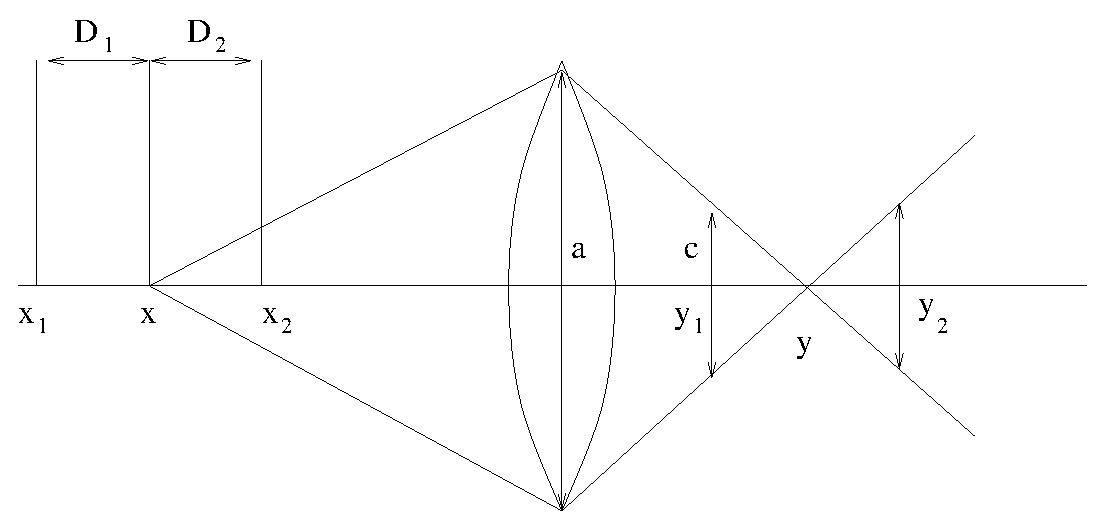
\includegraphics[width=0.9\textwidth]{FIGURES/depthoffield}
  \end{center}
  Controlled by aperture size and focal length.
\end{frame}

\section{Stereo}


\begin{frame}
  \frametitle{Multiple View Correspondences}
  \begin{center}
    \includegraphics[width=0.9\textwidth]{FIGURES/stereo}
  \end{center}
  If we can recover $x'$ from $x$ we can recover depth.
\end{frame}

\begin{frame}
  \frametitle{Image Correspondence}
  \begin{center}
    \includegraphics[width=0.9\textwidth]{IMAGES/stereo2images}
  \end{center}
  How do we match points from image 1 to image 2: you should have seen some of it with Kim,
  but this is not the end of the story!
\end{frame}


\begin{frame}
  \frametitle{Epipolar Constraints}
  \begin{center}
    \includegraphics[width=0.9\textwidth]{FIGURES/epipolarconstraint}
  \end{center}
  \begin{itemize}
  \item    Potential match for $x$ must lie in corresponding line $l'$
  \item  Potential match for $x'$ must lie in corresponding line $l$
  \end{itemize}  
\end{frame}


\begin{frame}
  \frametitle{Epipolar Constraints}
  \begin{center}
    \includegraphics[width=0.9\textwidth]{FIGURES/epigeom}
  \end{center}
  \begin{itemize}
  \item  Line connecting $O$ and $O'$: \myemph{baseline}
  \item Plane through baseline $x$ and $x'$: \myemph{Epipolar Plane}
  \item Epipoles: intersection of baseline and image planes:
    projection of the other camera center.
  \item Epipolar Lines - intersections of epipolar plane with image
    planes (always come in corresponding pairs)
  \end{itemize}  
\end{frame}


\begin{frame}
  \frametitle{Example: Converging cameras}
  \begin{center}
     \includegraphics[width=0.9\textwidth]{FIGURES/convergecam}
  \end{center}
\end{frame}

\begin{frame}
  \frametitle{Calibrated Case}
   \begin{center}
    \includegraphics[width=0.65\textwidth]{FIGURES/epicalibrated}
  \end{center}
  Camera parameters known for the two cameras: calibration matrices $K$ and $K'$\\
\end{frame}

\begin{frame}
  \begin{itemize}
  \item  $x$ and $x'$ (in 3D coords but not the same)  are related by rotation and translation.
    $$x' = R(x-\bt)$$
  \item Their homogeneous coordinates $y$ and $y'$ are related by a simple matrix $E$ built from $R$ and $t$
    $$
    y^T E y = 0.
    $$
  \item $E$ is called the \myemph{essential matrix} (Longuet-Higgins 1981).
  \item $E$ can be estimated from images.
  \item The position and orientation of camera 1 vs camera 2 (i.e.,
    $R$ and $\bt$) can be recovered from $E$.
  \end{itemize}
\end{frame}

\begin{frame}
  \frametitle{Note on the geometric transformation between image 1 and
    image2}
  \begin{itemize}
  \item The transformation between $y$ and $y'$ is not linear: it is
    an \myemph{homography} between the 2 image planes: 
  \item An homography conserves straight lines, but not parallelism. 
  \item Two parallel lines intersect at infinity: after an homography they may intersect at finite distance.
  \end{itemize}
\end{frame}


\begin{frame}
   \frametitle{Uncalibrated Case}
   \begin{itemize}
   \item No way to directly compare $x$ and $x'$: they relate through
     the unknown transformations $K$ and $K'$.
   \item A relation however still exists (Faugeras, Luong, 1992)
     $$
     y^T \udesc{F}{K^{-\top} E K'^{-1}} y =0
     $$
   \item $F$ is called the \myemph{fundamental matrix}. 
   \item Though $K$ and $K'$ are unknown $F$ can be \myemph{esitimated}
     (complicated) thus used for the correspondence problem!
   \item {\small $K^\top$ is the transposed of $K$: inverse row and line indices.
     For a vector in column, write it in line.}
   \item {\small $K^{-1}$ is the inverse of $K$: provides the inverse change
     of coordinates from unnormalized to normalized image coordinate.}
   \item {\small $K^{-\top}$ means inverse of the transposed matrix: The same
     as transposed of the inverse.}
   \end{itemize}
\end{frame}



\begin{frame}
   \begin{center}
    \includegraphics[width=\textwidth]{IMAGES/tired}
  \end{center}
\end{frame}

\end{document}


